\documentclass{beamer}

\usepackage{amsthm}
\usepackage[utf8]{inputenc}
\usepackage[T1]{fontenc}
\usepackage[brazil]{babel}
\usepackage[export]{adjustbox}
\usepackage{listings}
\usepackage{fontspec}
\usepackage{color}

\definecolor{pblue}{rgb}{0.13,0.13,1}
\definecolor{pgreen}{rgb}{0,0.5,0}
\definecolor{pred}{rgb}{0.9,0,0}
\definecolor{pgrey}{rgb}{0.46,0.45,0.48}

\lstset{language=Java,
  showspaces=false,
  showtabs=false,
  breaklines=true,
  showstringspaces=false,
  breakatwhitespace=true,
  commentstyle=\color{pgreen},
  keywordstyle=\color{pblue},
  stringstyle=\color{pred},
  basicstyle=\ttfamily,
}


\usetheme{Madrid}
\usecolortheme{beetle}
\usefonttheme{professionalfonts}

\setmainfont{Oswald}

\lstset{basicstyle=\ttfamily,breaklines=true}
\beamertemplatenavigationsymbolsempty

\begin{document}

\selectlanguage{brazil}
\title[MergeSort]{MergeSort}
\author{Prof. Andrey Masiero}

\begin{frame}[plain,noframenumbering]
  \titlepage
\end{frame}

\begin{frame}[plain,noframenumbering]
  \frametitle{Agenda}
  \tableofcontents
\end{frame}

\section{MergeSort}

\begin{frame}
	\frametitle{MergeSort}
    \begin{itemize}[<+->]
        \item Dividir: transformar os dados em pequenos subproblemas;
        \item Conquistar: Classificar os pequenos subproblemas resolvendo-os;
        \item Combinar: Juntar os subproblemas em um único conjunto classificado.
    \end{itemize}
\end{frame}

\begin{frame}
    \frametitle{MergeSort}
    \begin{itemize}[<+->]
        \item O vetor inicial é dividido ao meio até que existam apenas pares de elementos;
        \item Cada par é ordenado e depois são agrupados com outro par, em um vetor ordenado de quatro elementos;
        \item E assim é realizado o processo .
    \end{itemize}
\end{frame}

\begin{frame}
    \frametitle{MergeSort}
    \begin{itemize}[<+->]
        \item O vetor inicial é dividido ao meio até que existam apenas pares de elementos;
        \item Cada par é ordenado e depois são agrupados com outro par, em um vetor ordenado de quatro elementos;
        \item E assim é realizado o processo .
    \end{itemize}
\end{frame}

\begin{frame}
    \frametitle{MergeSort}
    \centering
    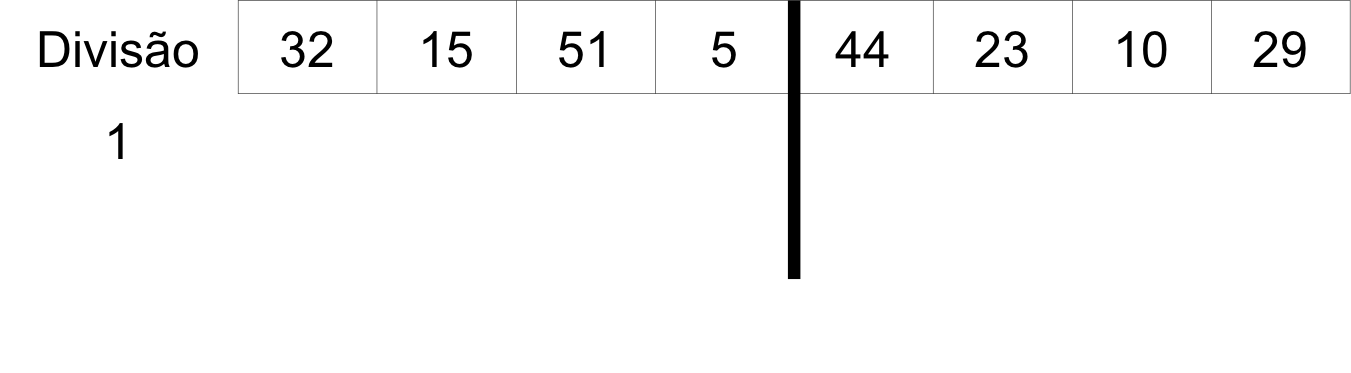
\includegraphics[scale=0.5]{images/1.png}
\end{frame}

\begin{frame}
    \frametitle{MergeSort}
    \centering
    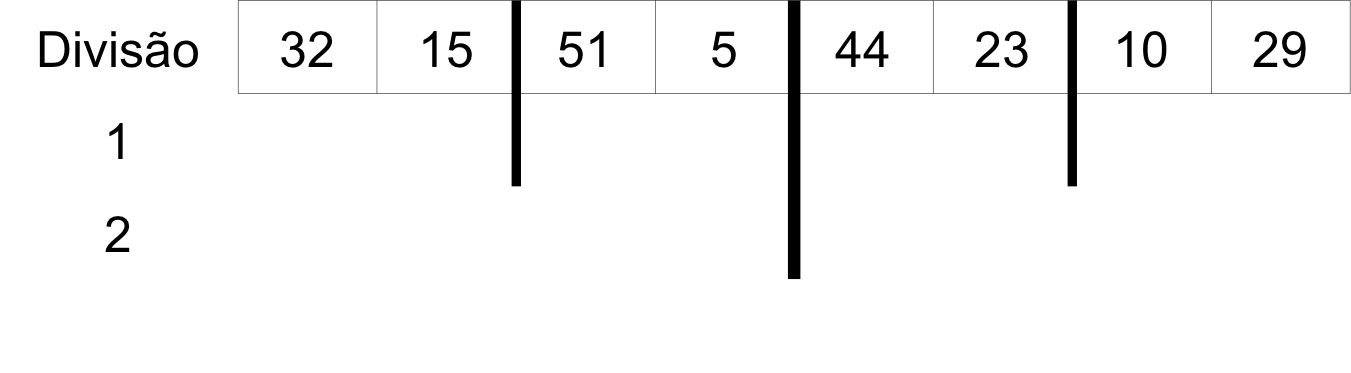
\includegraphics[scale=0.5]{images/2.png}
\end{frame}

\begin{frame}
    \frametitle{MergeSort}
    \centering
    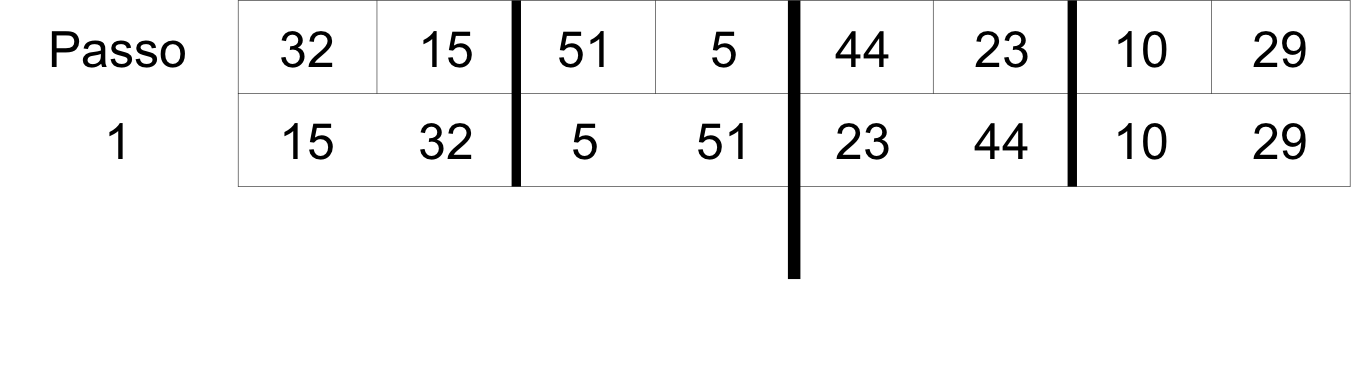
\includegraphics[scale=0.5]{images/3.png}
\end{frame}

\begin{frame}
    \frametitle{MergeSort}
    \centering
    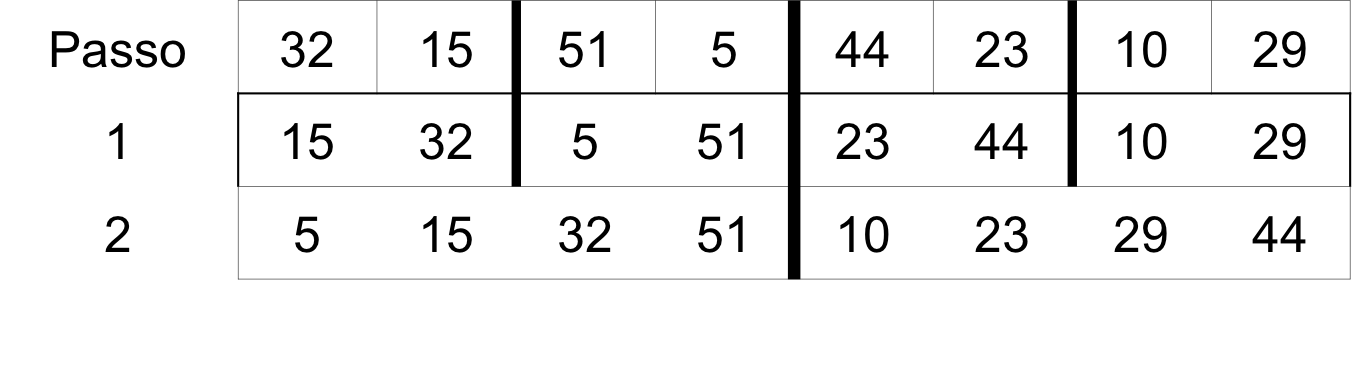
\includegraphics[scale=0.5]{images/4.png}
\end{frame}

\begin{frame}
    \frametitle{MergeSort}
    \centering
    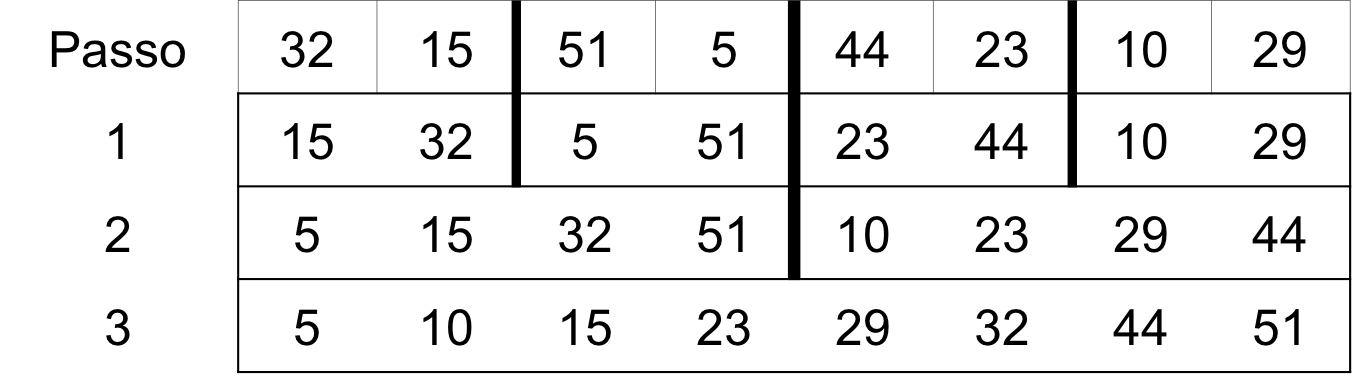
\includegraphics[scale=0.5]{images/5.png}
\end{frame}

\begin{frame}
	\frametitle{Algoritmo de Ordenação}
    \centering
    \lstinputlisting[language=Java]{src/sort.java}
\end{frame}

\begin{frame}
	\frametitle{Método Merge}
    \centering
    \lstinputlisting[language=Java]{src/merge.java}
\end{frame}

\begin{frame}
	\frametitle{Método Merge}
    \centering
    \lstinputlisting[language=Java]{src/merge2.java}
\end{frame}

\section{Exercícios}

\begin{frame}
    \frametitle{Exercícios}

    \begin{enumerate}
        \item Implemente o MergeSort.
        \item Teste os algoritmos em um programa principal, com o seguintes vetores:
        \begin{enumerate}
            \item 42, 21, 37, 75, 98, 11, 50, 63
            \item 88, 15, 27, 55, 44, 38
            \item 12, 81, 75, 37, 47, 25, 34
            \item 48, 11, 88, 33, 57, 12, 18, 87, 54, 8
        \end{enumerate}
    \end{enumerate}
\end{frame}

\section{Referências}

\begin{frame}
    \frametitle{Referências Bibliográficas}
    \begin{enumerate}
        \item Cormen, Thomas H., Charles E. Leiserson, Ronald L. Rivest, and Clifford Stein. ``Introduction to algorithms second edition.'' (2001).
        \item Tamassia, Roberto, and Michael T. Goodrich. ``Estrutura de Dados e Algoritmos em Java.'' Porto Alegre, Ed. Bookman 4 (2007).
        \item Ascencio, Ana Fernanda Gomes, and Graziela Santos de Araújo. ``Estruturas de Dados: algoritmos, análise da complexidade e implementações em JAVA e C/C++.'' São Paulo: Perarson Prentice Halt 3 (2010).
    \end{enumerate}
\end{frame}

\end{document}
